








\ps{I'm thinking an intro to globular clusters, then to modelling GCs with discussion of binaries,
	then to observations of binaries in GC}

\section{Globular Clusters}

Globular clusters (GCs) are dense, spheroidal collection of stars bound by their own self-gravity.
GCs are found in most galaxies, with the Milky Way hosting roughly 150, mostly located in the outer
halo. GCs typically represent some of the oldest stellar populations in the universe and are usually
in excess of 10 billion years old. Globular clusters were thought to have formed from a single giant
molecular cloud, resulting in a single coeval population of star with identical abundances. While
modern observation shave revealed that many clusters in fact have multiple independent population
with difference elemental abundances, most globular clusters are still well-approximated by a single
simple stellar population.

The dynamics of a cluster are almost entirely described by the gravitational interactions between
object in the cluster.

Any nice review paper I can cite or something similar?

Mention mass segregation

\subsection{Binaries in Globular Clusters}


In general, the binary systems found within present-day clusters differ significantly from the field
binaries that are more easily observed. In particular, we expect to little no long-period binaries,
on account of them being ionized by the frequent interactions with other cluster members. We
frequently use the terms "hard" and "soft" to describe binaries where "soft binaries" have a binding
energy comparable to the average kinetic energy of a cluster member while "hard binaries" have
larger binding energy. Due to the frequent interactions within clusters we expect that all soft
binaries have long since been ionized by the present-day leaving only a population of hard binaries
with a truncated period distribution compared to field binaries.
\ps{Cite some papers here}

\paragraph{}
Binary Burning: \citet{Chatterjee2013}


Black Hole Burning: \citet{Kremer2019}
\paragraph{}


Some dynamical effects of binaries, mention that we're focusing on hard binaries that we can treat
as point masses, not so much the long-period binaries that provide significant energy through
hardening during interactions.

The primary way that binaries can effect the dynamics of a cluster is through three-body
interactions with other cluster members. When a single star (or another binary) interacts with a
binary system at a close enough range, the binary system will "tighten", imparting some of its
energy to the ejected star. Through this process binary systems can act as a reserve of kinetic
energy for a cluster and are thought to be one of the primary mechanisms through which core-collapse
is halted in some clusters \citep{Chatterjee2013}. Because the models that we will be focusing on do
not model individual objects within the cluster we will instead focus of the second way that
binaries can effect the dynamics of a cluster.

Because binaries are tightly bound, for all interactions except for the very closest, they
effectively act as a single point mass equal to the sum of each component's mass. In this way,
binaries can affect cluster dynamics in much the same way that a large population of heavy remnants
might. Much like black holes and neutron stars, binary systems will migrate to the centre of a
cluster due to the effect of mass-segregation. \citet{Kremer2019} found that a central population of
black holes can fulfill a similar role to binary systems in halting core collapse by injecting
kinetic energy through two-body interactions within the core of the cluster. This same mechanism
could apply with tightly-bound binary systems that have mass-segregated to the centre of the
cluster. This predicted increase in binary fraction as you get closer to the centre of a cluster is
also seen in observations \ps{cite something here, sollima? giersz? }.

\subsection{Observations of Binary Stars in Globular Clusters}

\paragraph{}
In general, there are two methods used to detect binaries within globular clusters: high-precision
photometric observations and radial velocity surveys.

\paragraph{}
High-precision photometry can be used to detect binaries along the main sequence which have a
significant difference in the mass of their components ( typically these systems have a mass ratio,
$q$, larger than $0.5$). These systems will appear to be raised above the main-sequence when plotted
on a colour-magnitude diagram as their colour will match that of a typical main-sequence star
however their luminosity will be the sum of both components. Figure
\ref{fig:1/main_sequence_binaries} shows the main-sequence of the cluster NGC 2298, the binary stars
in this cluster are visible above the main-sequence according to their mass ratio.
\citet{Milone2012} performed high-precision photometry on several globular clusters using the Hubble
Space Telescope's (HST) Advanced Camera for Surveys and was able to place strong constraints on the
binary fraction for binaries with a mass ratio above $q=0.5$. This method allows for large studies
of binary populations in GCs without the need for dedicated observations but suffers from an
inherent bias towards systems with high mass ratios. Systems with mass ratios below $q=0.5$ are
typically too close to the regular main-sequence to confidently classify as binaries (see Figure
\ref{fig:1/main_sequence_binaries}). This means that studies which employ this method must assume an
underlying mass-ratio distribution if they wish to place any limits on the overall binary fraction
of a cluster.


\begin{figure}
	\centering
	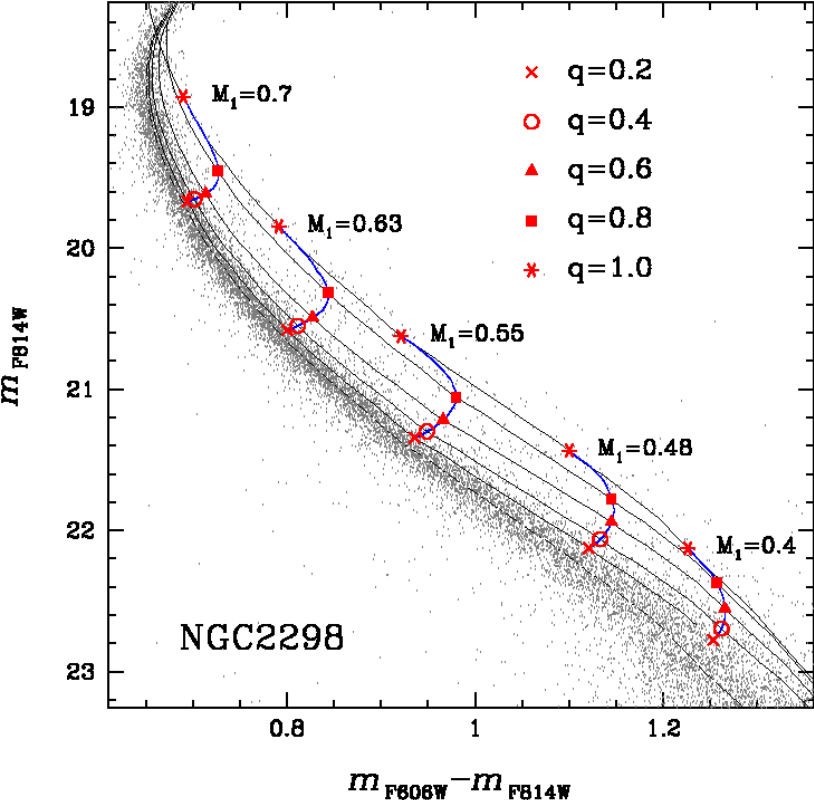
\includegraphics[width=0.8\textwidth]{"./figures/main_sequence_binaries.pdf"}
	\label{fig:1/main_sequence_binaries}
\caption{\ps{TODO: write proper caption} Reproduced from Figure 1 of \citet{Milone2012}.}
\end{figure}


Large-scale campaigns to measure the radial velocities for many stars in a cluster over several
epochs are another method which can be used to detect binaries in GCs. Systems which are found to
have periodically varying radial velocities can typically be confidently classified as binary
systems. \citet{Giesers2019} used the MUSE integral field spectrograph installed at the European
Southern Observatory's Very Large Telescope to observe several GCs and reported the results for NGC
3201. Integral field spectrographs provide spatially resolved spectra for the entire field of view
of the detector which enables far more time-efficient surveys than previous methods. Because this
methods measure radial velocities and periods, it can be used to constrain most of a binary system's
orbital parameters allowing us to verify our assumptions \ps{does it validate them? some binaries
	with periods up to 1000 days there?} about the period distributions of binaries in globular
clusters. \ps{grab a figure from the MUSE paper with period distribution?}



\section{Modelling Globular Clusters}

\paragraph{}

\ps{clean this up}

When modelling globular clusters, there are generally two approaches you can take. The first is to
model the entire evolutionary history of the cluster from initial conditions to the present. The
most commonly employed versions of these "evolutionary models" are direct N-body integration (see
for example \citet{Baumgardt2017a}) which directly calculate the gravitational interactions between
each object in the cluster and Monte-Carlo models (see \citet{Rodriguez2021} or \cite{Hypki2013})
which approximate the gravitational interactions between object according to the method of
\citet{Henon1971}. While these models provide insight into the dynamical history of the cluster,
they are very computationally expensive with even the fastest models taking on the order of a day
to model a realistic globular cluster \citep{Rodriguez2021}.

The second approach is to model just the present-day conditions of the cluster. These models, which
we call "equilibrium models", capture none of the dynamical history of the cluster but fully
describe the present-day state of the cluster and are orders of magnitude faster to compute with
typical models being on the order of a second.

These equilibrium models are much less computationally demanding than evolutionary models (N-body or
Monte Carlo models). Their relative efficiency allows us to explore a significantly larger parameter
space when fitting the models to observations to constrain the present-day properties of a cluster.
In particular, it is worth highlighting that by using equilibrium models we are able to vary the
stellar mass function of the cluster as well as the black hole and remnant retention fractions with
more flexibility than what might be possible with evolutionary models, due to the computational cost
of computing extensive grids of evolutionary models with many parameters varied in the initial
conditions (e.g. various stellar initial mass functions, initial cluster radii, masses, etc.).

The comparative efficiency of these models further enables the use of statistical fitting techniques
like MCMC or Nested Sampling which would be prohibitively expensive to use with evolutionary models.
This means that instead of a computing a grid of models and finding the "best-fitting" model we can
instead recover posterior distributions for key cluster parameters.

In this work we use the \code{LIMEPY} family of models presented by \citet{Gieles2015}. In their
current implementation, these models assume that all objects within the cluster are single and make
no attempt to model the dynamical effects of stellar multiplicity. In this project we adapt these
models to incorporate some of the effects of binary stars under the assumption that all long-period
binaries have been ionized by the present-day.


The \code{LIMEPY} models are a set of distribution function based equilibrium models that are
isothermal for the most bound stars near the cluster centre and described by polytropes in the outer
regions near the escape energy. The models have been extensively tested against $N$-body models
\citep{Zocchi2016, Peuten2017} and are able to effectively reproduce the effects of mass
segregation. Their suitability for mass modelling globular clusters has been tested on mock data
\citep{Henault-Brunet2019} and they have recently been applied to real datasets as well
\citep[e.g.][]{Gieles2018, Henault-Brunet2020}.



The input parameters needed to compute our models include the central concentration parameter $W_0$,
the truncation parameter $g$\footnote{Woolley models \citep{Woolley1954} have $g=0$, King models
	\citep{King1966} $g=1$, and Wilson models \citep{Wilson1975} $g=2$.}, the anisotropy radius $r_a$
which determines the degree of radial anisotropy in the models, $\delta$ which sets the mass
dependence of the velocity scale and thus governs the degree of mass segregation, and finally the
specific mass bins to use as defined by the mean stellar mass ($m_j$) and total mass ($M_j$) of each
bin, which together specify the stellar mass function. In order to scale the model units into
physical units, the total mass of the cluster $M$ and a size scale (the half-mass radius of the
cluster $r_h$) are provided as well.

